\documentclass[conference]{IEEEtran}
\IEEEoverridecommandlockouts
% The preceding line is only needed to identify funding in the first footnote. If that is unneeded, please comment it out.
\usepackage{cite}
\usepackage{amsmath,amssymb,amsfonts}
\usepackage{algorithmic}
\usepackage{graphicx}
\usepackage{textcomp}
\usepackage{xcolor}
\usepackage[brazilian]{babel}
\usepackage[utf8]{inputenc}
\usepackage[T1]{fontenc}
\def\BibTeX{{\rm B\kern-.05em{\sc i\kern-.025em b}\kern-.08em
    T\kern-.1667em\lower.7ex\hbox{E}\kern-.125emX}}
\begin{document}

\title{Particle Swarm Optimization}

\author{Bruno Lopes}
\maketitle

\begin{abstract}
teste

\end{abstract}

\section{INTRODUÇÃO}
teste

\section{Referencial Teórico}
	
	
	\begin{figure}[htbp]
	\centerline{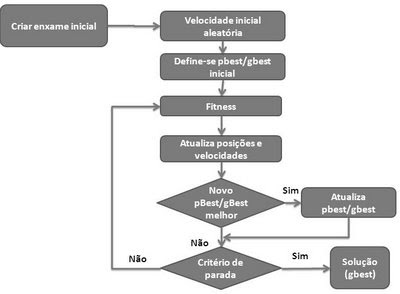
\includegraphics[scale=0.4]{pso_algoritmo.JPG}}
	\caption{Fluxograma-Algoritmo PSO}
	\label{fig}
	\end{figure}
	
	
\section{Metodologia Experimental}
    
  
\section{Resultado e Discussão}

   
    
\section*{Conclusão}

  

\begin{thebibliography}{00}

\bibitem{b1} 

\end{thebibliography}
\end{document}
